\chapter{Abbildungen}
\begin{sidewaysfigure}
	\centering 
	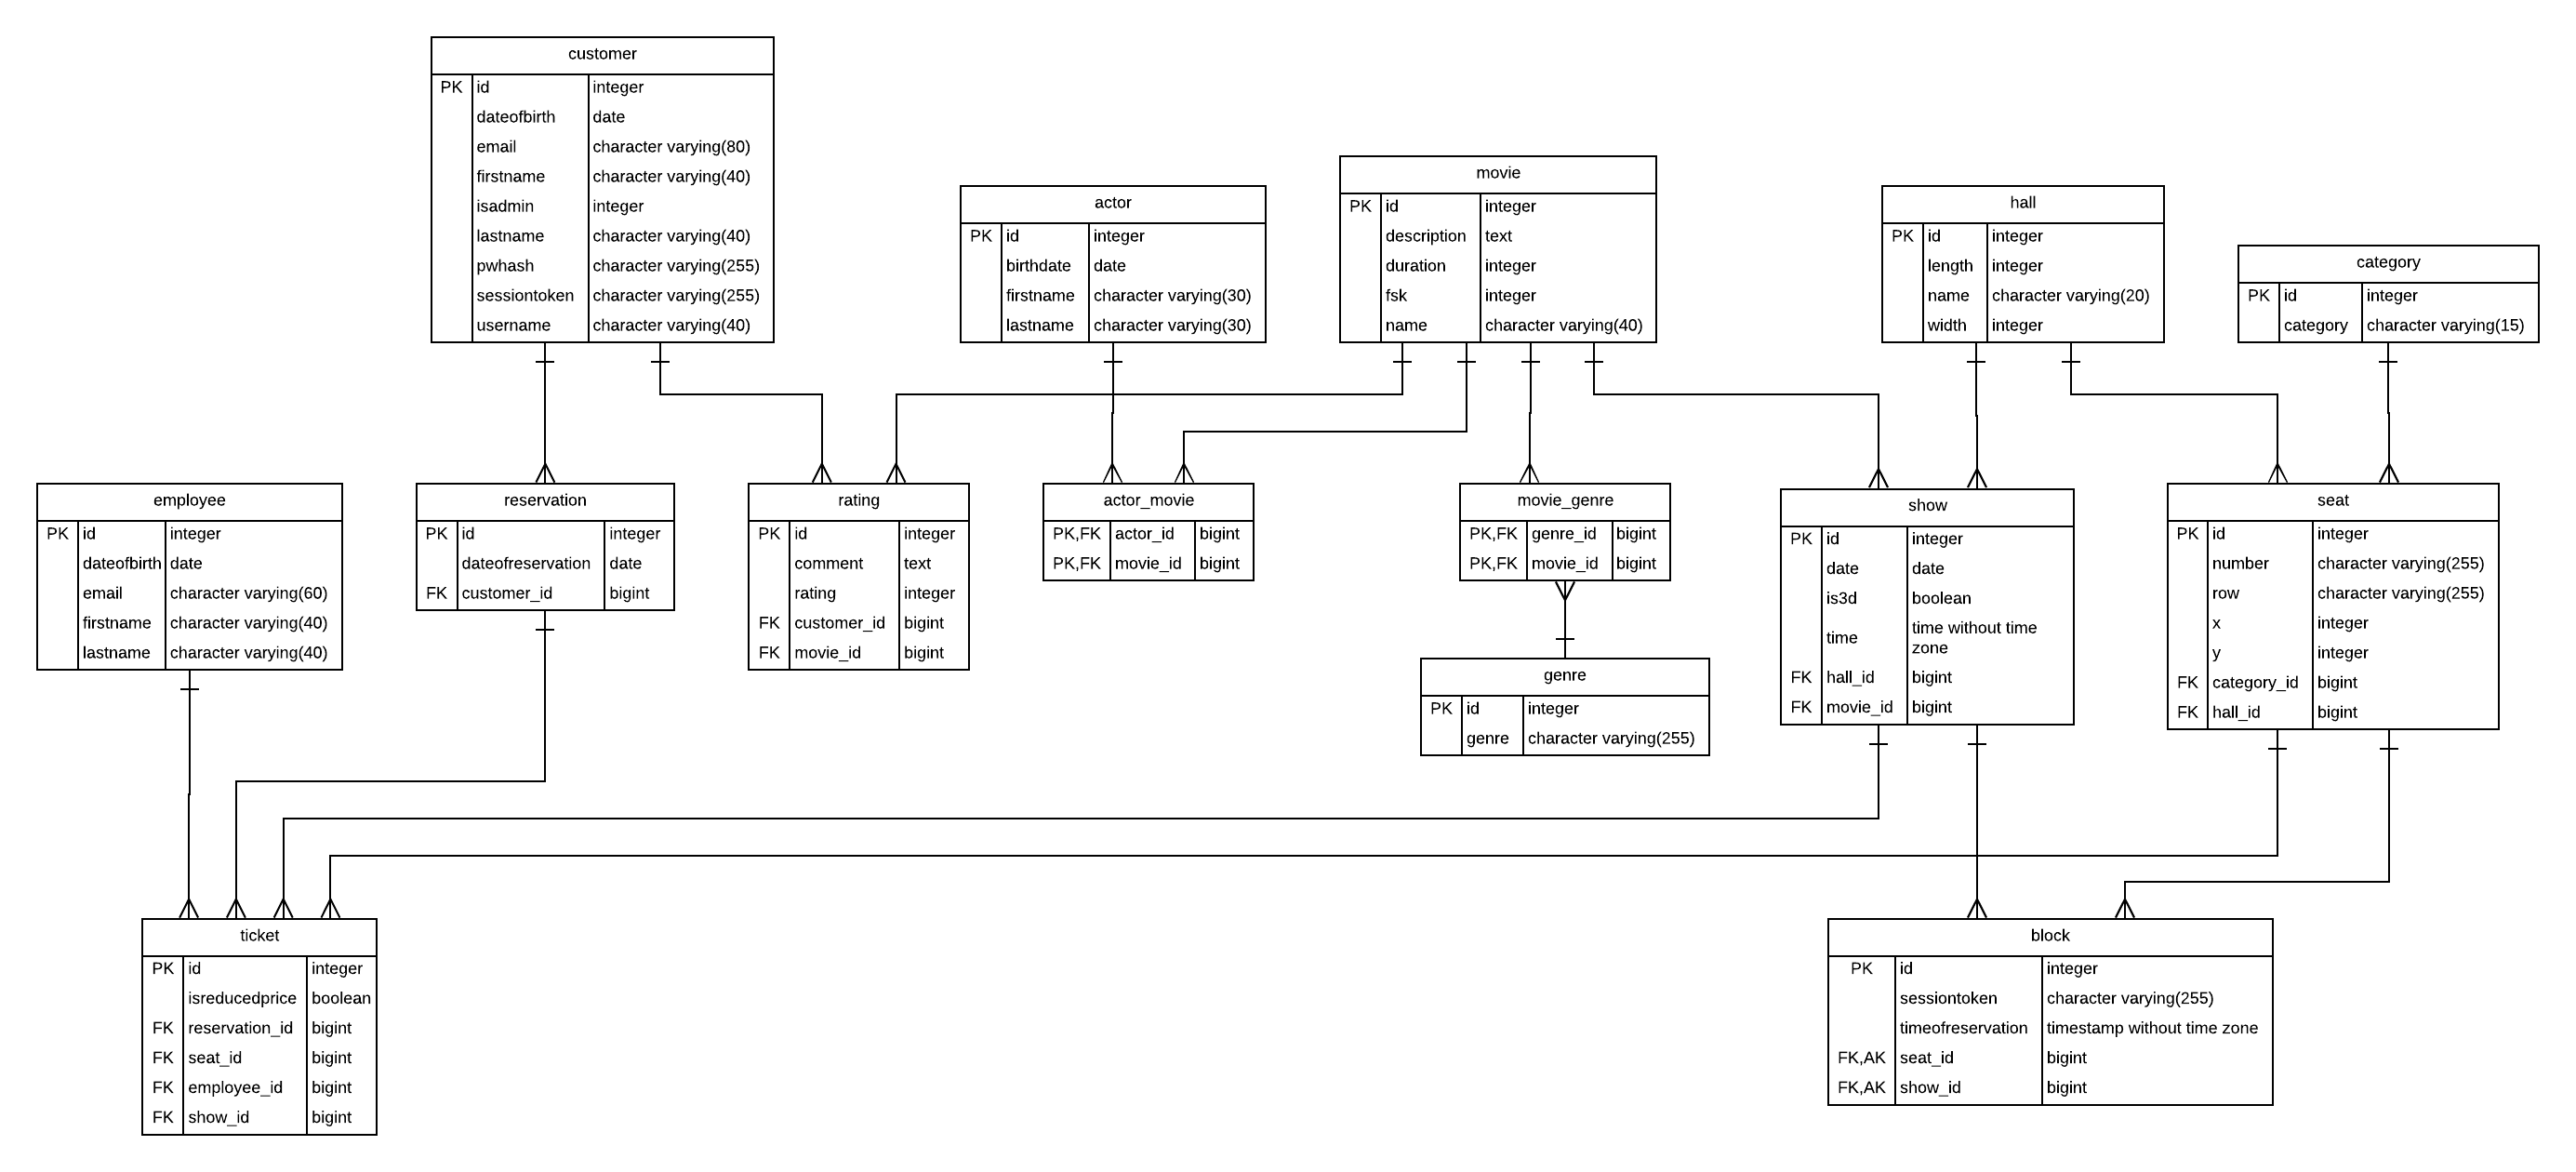
\includegraphics[keepaspectratio, width=1.0\textwidth, height=1.0\textheight]{img/ER-Modell}
	\captionsetup{format=hang}
	\caption{\acs{ER-Modell} der Datenbank}
	\small Quelle: eigene Darstellung mittels \url{https://www.lucidchart.com/}
	\label{fig:Anhang_ER-Modell}
\end{sidewaysfigure}

\chapter{Quellcode}
\begin{minipage}{\linewidth}
	\begin{lstlisting}[style=lstJava]
	public static MovieTo createMovieTo ( Movie entity, boolean withShow )
	{
	if ( null != entity )
	{
	MovieTo movieTo = new MovieTo();
	movieTo.setId(entity.getId());
	movieTo.setDescription(entity.getDescription());
	movieTo.setFsk(entity.getFsk());
	movieTo.setDuration(entity.getDuration());
	movieTo.setName(entity.getName());
	movieTo.setGenres(createGenreTos(entity.getGenres()));
	movieTo.setRatings(createRatingTos(entity.getRatings()));
	if ( withShow )
	{
	movieTo.setShows(createShowTos(entity.getShows(), false));
	} // end withSow
	movieTo.setActors(createActorTos(entity.getActors()));
	return movieTo;
	}  // end if null
	return null;
	}
	\end{lstlisting}
	\captionof{lstlisting}{Erstellen eines Movie-\acs{DTO} aus einer Movie-Entität mit Hilfe des eigen erstellten EntityToToHelper}
	\label{lst:EntityToToHelper_movie}
\end{minipage}

\begin{minipage}{\linewidth}
	\begin{lstlisting}[style=lstJava]
	public static Movie createMovieEntity ( MovieTo transferObject, boolean withShow )
	{
		if ( null != transferObject )
		{
			Movie movie = new Movie();
			movie.setId(transferObject.getId());
			movie.setActors(createActorEntities(transferObject.getActors()));
			movie.setDescription(transferObject.getDescription());
			movie.setFsk(transferObject.getFsk());
			movie.setDuration(transferObject.getDuration());
			movie.setName(transferObject.getName());
			movie.setRatings(createRatingEntities(transferObject.getRatings()));
			if ( withShow )
			{
				movie.setShows(createShowEntities(transferObject.getShows(), false));
			}
			movie.setGenres(createGenreEntities(transferObject.getGenres()));
			return movie;
		}
		return null;
	}
	\end{lstlisting}
	\captionof{lstlisting}{Erstellen einer Movie-Entität aus einem Movie-\acs{DTO} mit Hilfe des eigen erstellten ToToEntityHelper}
	\label{lst:ToToEntityHelper_movie}
\end{minipage}